\documentclass[11pt,a4paper]{article}
\usepackage[margin=2.5cm]{geometry}
\usepackage{booktabs}
\usepackage{hyperref}
\usepackage{amsmath}
\usepackage{amssymb}
\usepackage{graphicx}
\usepackage{caption}
\usepackage{subcaption}
\usepackage{listings}
\usepackage{xcolor}
\usepackage{natbib}
\usepackage{algorithm}
\usepackage{algpseudocode}
\usepackage{tikz}
\usetikzlibrary{decorations.pathreplacing}
\usepackage{amsthm}
\usepackage[skip=0.5\baselineskip]{parskip}

\theoremstyle{definition}
\newtheorem{definition}{Definition}
\theoremstyle{plain}
\newtheorem{lemma}{Lemma}

\definecolor{codegreen}{rgb}{0,0.6,0}
\definecolor{codegray}{rgb}{0.5,0.5,0.5}
\definecolor{codepurple}{rgb}{0.58,0,0.82}
\definecolor{backcolour}{rgb}{0.95,0.95,0.92}

\lstdefinestyle{mystyle}{
backgroundcolor=\color{backcolour},
commentstyle=\color{codegreen},
keywordstyle=\color{magenta},
numberstyle=\tiny\color{codegray},
stringstyle=\color{codepurple},
basicstyle=\ttfamily\footnotesize,
breakatwhitespace=false,
breaklines=true,
captionpos=b,
keepspaces=true,
numbers=left,
numbersep=5pt,
showspaces=false,
showstringspaces=false,
showtabs=false,
tabsize=2
}
\lstset{style=mystyle}

\title{\textbf{The Li-Chao Tree: Algorithm Specification and Analysis}}
\author{Li Chao}
\date{\today}

\begin{document}

\maketitle

\begin{abstract}
The Li-Chao tree (LICT) was first introduced in 2012 lecture materials as an efficient data structure for dynamic lower envelope maintenance. In the years since, it has achieved widespread adoption within the competitive programming community and has been incorporated into standard algorithm libraries, yet no formal specification has appeared in the peer-reviewed literature. This paper provides the definitive formalization of the Li-Chao tree, serving as both the official specification and an expansion of the original 2012 lecture materials. We present complete algorithmic specifications, establish formal correctness proofs, analyze theoretical complexity, and provide empirical performance characterization. The LICT offers distinct advantages in implementation simplicity, numerical stability, and extensibility to advanced variants such as persistence and line segments.
\end{abstract}

\section{Introduction}

Dynamic Lower Envelope maintenance is a fundamental problem in computational geometry with extensive applications. We focus on the Li-Chao tree (LICT), a data structure that maintains a set of linear functions while supporting insertion and query operations. The problem is defined as follows: given a dynamic set of linear functions $y = kx + b$, support efficient insertion of new lines and querying the minimum (or equivalently, maximum) value at arbitrary $x$ coordinates. This report focuses on minimum queries; maximum queries are obtained by negating line parameters.

Formally, we require a data structure supporting two operations:
\begin{enumerate}
\item \textbf{Add Line:} Insert a new line $y = kx + b$ into the structure.
\item \textbf{Query:} Given $x_0$, compute
\[
\min_{i} \{k_i x_0 + b_i\}
\]
over all lines currently in the structure.
\end{enumerate}

The structure also supports line segments (lines defined only on finite intervals \[x_l, x_r\]) in addition to infinite lines.

Both operations must execute in logarithmic time for acceptable performance at scale. The LICT provides $O(\log C)$ time per operation for minimum (or maximum) queries, where
\[
C = \frac{\text{coordinate range}}{\text{precision level}}
\]
represents the ratio of the coordinate range to the precision level. For integer coordinates with range $[0, 10^9]$, $C = 10^9$; for the same range with precision $10^{-6}$, $C = 10^{15}$.

\subsection{Background}

In 2012, the Li-Chao tree was presented informally in a lecture context.\footnote{The data structure is conventionally referred to as the ``Li-Chao tree'' in the literature and competitive programming community.} It subsequently gained widespread adoption within the competitive programming community. This paper formalizes the LICT and provides a comprehensive analysis of its properties and performance, with particular attention to extensibility features.

\subsection{Historical Note}

The Li-Chao tree originated in 2012, when the author first presented the structure in lecture materials for the Zhejiang Provincial Olympiad in Informatics (ZJOI). The algorithm emerged from the need for a data structure that could efficiently handle online line container problems while remaining simple enough to implement under competitive programming time constraints.

Following its introduction, the structure underwent significant evolution within the Competitive Programming community. Early implementations were shared informally through online forums and regional contest materials. By 2015, the algorithm had appeared in major competitive programming platforms, with practitioners developing various optimizations and extensions. The 2017 publication of a tutorial on Codeforces marked a turning point, establishing standardized terminology and implementation patterns.

Today, the Li-Chao tree is included in major competitive programming libraries including KACTL (KTH Algorithm Library) and CP-Algorithms, and has been applied in thousands of contest problems. Its sustained relevance over more than a decade demonstrates the structure's practical utility and the community's continued investment in its development.

\section{Related Work}\label{sec:related}

Several approaches exist for Dynamic Lower Envelope maintenance, each with distinct trade-offs in terms of time complexity, implementation complexity, and applicability constraints. We review these solutions to establish the context for the LICT.

Dynamic maintenance of geometric configurations has been studied extensively in computational geometry.

\subsection{Overmars and van Leeuwen (1981)}

Overmars and van Leeuwen \cite{overmars1981} presented foundational work on dynamic convex hull maintenance. Their data structure supports insertion and deletion of lines while maintaining the lower envelope, enabling efficient querying of the minimum value at any point.

Their approach uses a balanced binary search tree to explicitly maintain the convex hull. Each node stores a line, and the tree is ordered by slope. Intersection points between adjacent lines are computed to determine the hull structure. Queries take $O(\log n)$ time, while insertions and deletions require $O(\log^2 n)$ time. The space complexity is $O(n)$, storing each inserted line exactly once.

Their work established the theoretical framework for dynamic geometric data structures and demonstrated that logarithmic-time dynamic maintenance of the lower envelope is achievable.

\subsection{Monotonic Convex Hull Trick}

The monotonic convex hull trick addresses the special case where line slopes are inserted in monotonically increasing or decreasing order.

When insertions arrive in order of monotonically increasing (or decreasing) slopes, a deque-based approach achieves $O(1)$ amortized time per insertion and $O(1)$ amortized time per query. This variant, widely used in dynamic programming optimization, maintains the convex hull incrementally without requiring balanced tree structures. However, the monotonicity restriction limits its applicability to problems where line slopes are known to follow a specific order.

\subsection{Dynamic Convex Hull Trick}

For arbitrary insertion sequences without monotonicity constraints, a balanced binary search tree maintains the hull explicitly. Each insertion and query requires $O(\log n)$ amortized time. The implementation complexity stems from the need to compute and maintain intersection points between adjacent lines in the hull.

The Dynamic CHT requires computing intersection points between adjacent lines in the hull as $x_{\text{intersect}} = \frac{b_2 - b_1}{k_1 - k_2}$, necessitating careful handling of division by zero (parallel lines), integer overflow, and sign conventions for floored division.

\section{Overview}\label{sec:lichao}

This section presents the Li-Chao tree.

\subsection{Algorithmic Approach}

The LICT offers a fundamentally different approach based on implicit envelope maintenance through interval subdivision. Rather than tracking the convex hull geometry explicitly, the structure maintains the best line at each interval midpoint, recursively partitioning the query range.

Each node in the tree represents an interval $[\text{left}, \text{right}]$ and stores one line. During insertion, a line is \emph{routed} through the tree following a single path from root to leaf. At each node on this path, the new line is compared with the currently stored line. The line that achieves the lower value at the midpoint $\text{mid} = (\text{left}+\text{right})/2$ is \emph{stored} at that node; the suboptimal line continues downward to be routed through the appropriate child subtree.

\textbf{Key invariant (local optimality).} A line stored at a node achieves the minimum value among all lines routed through that node at the midpoint of the node's interval. Formally, for node with interval $[\text{left}, \text{right}]$ and midpoint $\text{mid} = (\text{left}+\text{right})/2$, the stored line minimizes $kx + b$ at $x = \text{mid}$ among all lines routed to that node.

\begin{figure}[h]
\centering
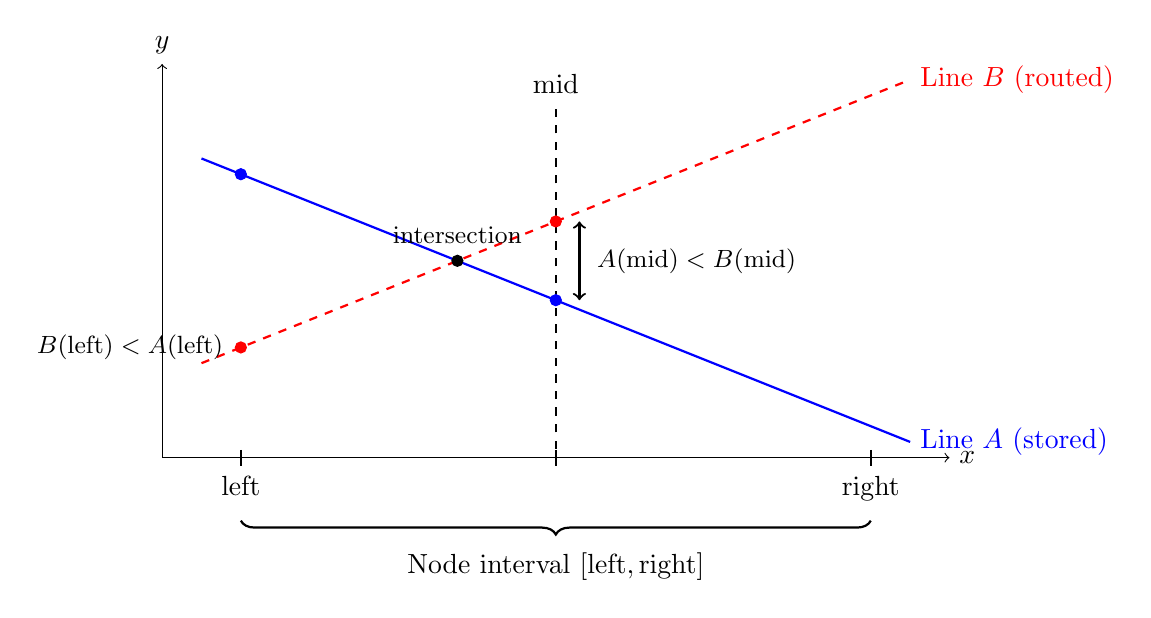
\begin{tikzpicture}[scale=1.0]
% Draw axes
\draw[->] (0,0) -- (10,0) node[right] {$x$};
\draw[->] (0,0) -- (0,5) node[above] {$y$};

% Draw interval [left, right] on x-axis
\draw[thick] (1,0.1) -- (1,-0.1) node[below] {\text{left}};
\draw[thick] (9,0.1) -- (9,-0.1) node[below] {\text{right}};
\draw[thick, decorate, decoration={brace, amplitude=5pt, mirror}] (1,-0.8) -- (9,-0.8) node[midway, below=8pt] {Node interval $[\text{left}, \text{right}]$};

% Draw midpoint
\draw[thick, dashed] (5,-0.1) -- (5,4.5) node[above] {$\text{mid}$};
\draw[thick] (5,0.1) -- (5,-0.1);

% Draw two intersecting lines
% Line A: y = -0.4x + 4 (stored at node - lower at midpoint, higher at left)
\draw[thick, blue] (0.5,3.8) -- (9.5,0.2) node[right] {Line $A$ (stored)};
% Line B: y = 0.4x + 1 (routed to left child - lower at left, higher at mid)
\draw[thick, red, dashed] (0.5,1.2) -- (9.5,4.8) node[right] {Line $B$ (routed)};

% Mark intersection point (at x = 3.75)
\filldraw[black] (3.75,2.5) circle (2pt);
\node[above] at (3.75,2.6) {\small intersection};

% Mark values at midpoint (x = 5)
\filldraw[blue] (5,2.0) circle (2pt);
\filldraw[red] (5,3.0) circle (2pt);
\draw[thick, <->] (5.3,2.0) -- (5.3,3.0);
\node[right] at (5.4,2.5) {\small $A(\text{mid}) < B(\text{mid})$};

% Mark values at left endpoint (x = 1)
\filldraw[blue] (1,3.6) circle (2pt);
\filldraw[red] (1,1.4) circle (2pt);
\node[left] at (0.9,1.4) {\small $B(\text{left}) < A(\text{left})$};
\end{tikzpicture}
\caption{Interval Advantage Line Diagram. The node stores Line $A$ because it achieves the lower value at the midpoint. Line $B$ is routed to the left child where it may be optimal.}
\label{fig:interval-advantage}
\end{figure}

Note that this is \emph{local} optimality only. Lines routed down other branches may achieve lower values at the midpoint, so the stored line is not necessarily globally optimal at that coordinate.

At query time, we traverse the path to $x_0$, evaluating all stored lines along the path. The minimum value encountered equals the lower envelope at $x_0$ because any line that could be optimal at $x_0$ is stored on this path.

Insertion proceeds as follows: if the new line yields a lower value at the midpoint, the lines are swapped and the suboptimal line continues down.

The appropriate child is determined by where the relative ordering changes. Let $f_\text{new}(x) = k_\text{new} x + b_\text{new}$ denote the new line and $f_\text{stored}(x) = k_\text{stored} x + b_\text{stored}$ denote the line currently stored at the node. Define boolean comparison values:
\begin{align*}
L &= [f_\text{new}(\text{left}) < f_\text{stored}(\text{left})] \\
M &= [f_\text{new}(\text{mid}) < f_\text{stored}(\text{mid})]
\end{align*}
where $[\cdot]$ denotes 1 if true and 0 if false. The child selection rule is:
\begin{equation*}
\text{child} =
\begin{cases}
\text{left} & \text{if } L \neq M \\
\text{right} & \text{if } L = M
\end{cases}
\end{equation*} This follows from the single-intersection property: if the ordering changes between $\text{left}$ and $\text{mid}$, the intersection point lies in $[\text{left}, \text{mid}]$; otherwise, it lies in $[\text{mid}, \text{right}]$.

Algorithms~\ref{alg:insert} and~\ref{alg:query} present the insertion and query procedures.

\begin{algorithm}[h]
\caption{LICT Line Insertion}
\label{alg:insert}
\begin{algorithmic}[1]
\Require Node pointer $node$, new line $new\_line$, interval $[l, r]$
\If{$node$ is null}
\State $node \gets \text{new Node}(new\_line)$
\State \Return
\EndIf
\State $mid \gets l + (r - l) / 2$
\State $lef \gets new\_line.eval(l) < node.line.eval(l)$
\State $midf \gets new\_line.eval(mid) < node.line.eval(mid)$
\If{$midf$}
\State swap($node.line$, $new\_line$)
\EndIf
\If{$l = r$}
\State \Return
\EndIf
\If{$lef \neq midf$}
\State \Call{Insert}{$node.left$, $new\_line$, $l$, $mid$}
\Else
\State \Call{Insert}{$node.right$, $new\_line$, $mid+1$, $r$}
\EndIf
\end{algorithmic}
\end{algorithm}

\begin{algorithm}[h]
\caption{LICT Query}
\label{alg:query}
\begin{algorithmic}[1]
\Require Node pointer $node$, query coordinate $x$, interval $[l, r]$
\Ensure Minimum value at coordinate $x$
\If{$node$ is null}
\State \Return $+\infty$
\EndIf
\State $mid \gets l + (r - l) / 2$
\State $val \gets node.line.eval(x)$
\If{$l = r$}
\State \Return $val$
\EndIf
\If{$x \leq mid$}
\State \Return $\min(val, \text{\Call{Query}{$node.left$, $x$, $l$, $mid$}})$
\Else
\State \Return $\min(val, \text{\Call{Query}{$node.right$, $x$, $mid+1$, $r$}})$
\EndIf
\end{algorithmic}
\end{algorithm}

\subsection{Theoretical Analysis}

We now present a formal analysis of the LICT's correctness and complexity.

\begin{definition}[Coordinate Universe]
The LICT operates on a discrete domain where $C = \frac{\text{coordinate range}}{\text{precision level}}$. The tree depth is $h = \lceil \log_2 C \rceil$.
\end{definition}

\subsubsection{Correctness}

We first establish the geometric intuition underlying the LICT's correctness. The key insight is that two distinct lines intersect at most once. This fundamental property of linear functions ensures that if a line yields a higher value at a midpoint, it can yield a lower value than the stored line on at most one side of the midpoint, never both.

\textbf{Why this maintains the lower envelope.} Consider two lines $A$ and $B$ compared at a node's midpoint:
\begin{itemize}
\item If $A$ achieves a lower value than $B$ at $\text{mid}$, but $B$ yields a lower value at one endpoint, then $B$ can only outperform $A$ on the side of $\text{mid}$ containing that endpoint (since two lines intersect at most once).
\item Therefore, $B$ is routed to exactly one child---the side where it might achieve a lower value.
\end{itemize}

This property guarantees that the suboptimal line need only be propagated down a single child path.

\begin{lemma}[Local Optimality Invariant]\label{lem:local-opt}
For any node $v$ with interval $[l, r]$ and midpoint $m = \lfloor(l+r)/2\rfloor$, the line stored at $v$ achieves the minimum value at $x = m$ among all lines that have been routed through $v$.
\end{lemma}

\begin{proof}
We proceed by induction on the sequence of insertions.

\textbf{Base case:} When the first line is inserted, it is stored at the root and all descendants are null. The invariant holds trivially.

\textbf{Inductive step:} Assume the invariant holds before inserting a new line $L_{\text{new}}$. Consider the insertion path from root to leaf. At each node $v$ along this path:
\begin{enumerate}
\item Let $L_{\text{stored}}$ be the line currently at $v$.
\item If $L_{\text{new}}(m) \geq L_{\text{stored}}(m)$, we keep $L_{\text{stored}}$ and route $L_{\text{new}}$ to a child. The invariant at $v$ remains satisfied.
\item If $L_{\text{new}}(m) < L_{\text{stored}}(m)$, we swap the lines, storing $L_{\text{new}}$ and routing $L_{\text{stored}}$ to a child. The invariant at $v$ is now satisfied by $L_{\text{new}}$.
\end{enumerate}
The routed line proceeds to exactly one child (determined by the intersection point location), so the inductive hypothesis applies to subtrees. By induction, the invariant holds after all insertions.
\end{proof}

\begin{lemma}[Query Correctness]\label{lem:query-correct}
For any query point $x_0 \in X$, the value returned by the query operation equals $\min_{i} \{k_i x_0 + b_i\}$ over all lines in the structure.
\end{lemma}

\begin{proof}
Consider any line $L$ in the structure and the query point $x_0$. Let $P$ be the unique root-to-leaf path whose intervals all contain $x_0$. Line $L$ follows exactly one root-to-leaf path $P_L$ during insertion.

We claim $L$ is evaluated at $x_0$ if and only if $x_0$ lies in the interval where $L$ is optimal among lines routed through some node on $P_L$. There are two cases:
\begin{enumerate}
\item If $P_L = P$, then $L$ is stored at some node on $P$ (specifically, at the deepest node where it achieved minimum at the midpoint), and is evaluated during the query.
\item If $P_L \neq P$, let $v$ be the deepest node common to both paths. Since $x_0$ is not in the child interval that $L$ was routed to, $x_0$ lies on the opposite side of the midpoint from where $L$ could potentially be better than the stored line. By the single-intersection property of lines, $L$ cannot be optimal at $x_0$.
\end{enumerate}
Thus, exactly those lines that could be optimal at $x_0$ are evaluated, and the minimum over evaluated lines equals the global minimum.
\end{proof}

\subsubsection{Complexity Analysis}

\begin{lemma}[Time Complexity]\label{lem:time-complexity}
Both insertion and query operations require $O(\log C)$ time.
\end{lemma}

\begin{proof}
The LICT is a binary tree of depth $h = \lceil \log_2 C \rceil = O(\log C)$.

For insertion: The new line follows exactly one root-to-leaf path. At each node, we perform: (1) $O(1)$ line evaluations ($kx + b$); (2) $O(1)$ comparisons; and (3) optionally a line swap. Each operation takes $O(1)$ time. With $O(\log C)$ nodes visited, total time is $O(\log C)$.

For query: The traversal follows one root-to-leaf path with $O(1)$ work per node (line evaluation and comparison). Total time is $O(\log C)$.
\end{proof}

\begin{lemma}[Space Complexity]\label{lem:space-complexity}
The LICT stores at most $O(n \log C)$ nodes in the worst case, where $n$ is the number of inserted lines.
\end{lemma}

\begin{proof}
Each line insertion creates at most one new node per level along its insertion path (when reaching a null child). The path length is $O(\log C)$. With $n$ insertions, the total number of nodes is at most $O(n \log C)$.
\end{proof}

\textbf{Pseudo-polynomial Nature.} We emphasize that the complexity $O(\log C)$ is pseudo-polynomial: it depends on the coordinate range parameter $C$, not solely on the input size $n$. For $w$-bit coordinates, $C \leq 2^w$, so $\log C \leq w$. When $w = O(\log n)$, this yields $O(\log n)$ time. However, for large coordinate ranges (e.g., 64-bit coordinates), the complexity is effectively $O(w) = O(1)$ relative to the coordinate bit width, though still pseudo-polynomial when measured against input bit complexity.

\textbf{Querying.} To query the minimum value at a coordinate $x_0$, we traverse the tree from root to leaf, following the path corresponding to the interval containing $x_0$. At each node, we evaluate the stored line at $x_0$ and keep track of the minimum value seen. The traversal proceeds to the left child if $x_0$ is in the left half of the current interval, or to the right child otherwise. When reaching a leaf (or a null child), we return the minimum value accumulated along the path. This traversal visits at most one node per tree level, yielding $O(\log C)$ query time.

\begin{itemize}
\item \textbf{Time Complexity:} $O(\log C)$ per operation, where $C = \frac{\text{coordinate range}}{\text{precision level}}$.
\item \textbf{Space Complexity:} At most $O(n \log C)$ nodes in the worst case when all lines follow disjoint paths through the tree. In practice, heavy node sharing occurs as lines with similar slopes traverse common paths, typically resulting in significantly lower memory usage.
\item \textbf{Key Characteristics:} No intersection calculations required; all decisions based on direct line evaluations ($kx+b$) at query points. This avoids the division operations ($\frac{b_2-b_1}{k_1-k_2}$) required by CHT for computing intersection points, which can suffer from precision issues when slopes are very close.
\end{itemize}

\textbf{Deletion.} Unlike the Dynamic CHT, which can support deletion of arbitrary lines in $O(\log n)$ amortized time, the standard LICT does not support efficient deletion. Removing a line would require traversing all nodes where that line might be stored and recomputing optimal lines from descendants, which requires $\Omega(n)$ time in the worst case. For applications requiring deletion, an alternative approach is reconstructing the tree periodically.

The LICT's complexity depends on the coordinate range rather than the number of lines. This provides consistent performance regardless of hull size, though it cannot exploit cases where the hull remains small relative to the number of insertions.

\begin{itemize}
\item \textbf{Time Complexity:} $O(\log C)$ per operation, where
\[
C = \frac{\text{coordinate range}}{\text{precision level}}.
\]
\item \textbf{Space Complexity:} At most $O(n \log C)$ nodes in the worst case when all lines follow disjoint paths through the tree. In practice, heavy node sharing occurs as lines with similar slopes traverse common paths, typically resulting in significantly lower memory usage.
\item \textbf{Key Characteristics:} No intersection calculations required; all decisions based on direct line evaluations ($kx+b$) at query points. This avoids the division operations
\[
\frac{b_2-b_1}{k_1-k_2}
\]
required by CHT for computing intersection points, which can suffer from precision issues when slopes are very close.
\end{itemize}

\subsection{Key Trade-offs}

The choice between these approaches involves several trade-offs:

\textbf{Performance versus simplicity.} The Dynamic CHT achieves faster query and insertion times, particularly when the hull remains small relative to the number of insertions. The LICT provides implementation simplicity and reduced code complexity at the cost of some performance. The LICT eliminates complex geometric calculations, reducing implementation time and probability of errors. This is particularly important in competitive programming and rapid prototyping contexts.

\textbf{Geometric versus combinatorial.} The Dynamic CHT relies on geometric calculations (intersection points as $\frac{b_2-b_1}{k_1-k_2}$) that require careful numerical handling, particularly when slopes are nearly equal. The LICT uses only basic arithmetic operations (multiplication and addition for $kx+b$ evaluations at query points), completely avoiding division and its associated precision concerns.

\textbf{Static versus extensible.} The Dynamic CHT's explicit hull structure makes extensions such as persistence and line segments difficult. The LICT's recursive tree structure naturally accommodates these extensions. Line segments (lines valid only on subranges $[l', r']$) integrate naturally. During insertion, when the current node interval $[l, r]$ lies entirely outside $[l', r']$, we skip that subtree. When $[l, r]$ lies entirely inside, we proceed normally. Otherwise, we recurse into both children. This limits the line's influence to its valid range without modifying the core algorithm. A segment $[x_l, x_r]$ decomposes into $O(\log C)$ canonical intervals; each interval requires a standard $O(\log C)$ line insertion, yielding
\[
O(\log^2 C)
\]
total time for line segment insertion.

\begin{figure}[h]
\centering
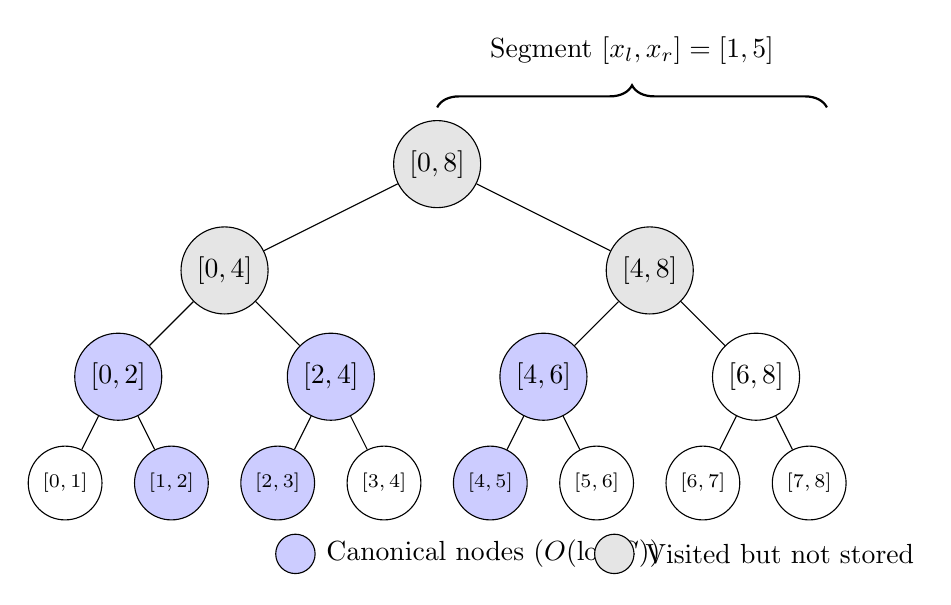
\begin{tikzpicture}[scale=0.9, level distance=1.5cm,
level 1/.style={sibling distance=6cm},
level 2/.style={sibling distance=3cm},
level 3/.style={sibling distance=1.5cm}]

% Tree structure showing segment decomposition
\node[draw, circle, fill=gray!20, minimum size=0.8cm] {$[0, 8]$}
child {node[draw, circle, fill=gray!20, minimum size=0.8cm] {$[0, 4]$}
child {node[draw, circle, fill=blue!20, minimum size=0.8cm] {$[0, 2]$}
child {node[draw, circle, fill=white, minimum size=0.6cm] {\scriptsize $[0,1]$}}
child {node[draw, circle, fill=blue!20, minimum size=0.6cm] {\scriptsize $[1,2]$}}
}
child {node[draw, circle, fill=blue!20, minimum size=0.8cm] {$[2, 4]$}
child {node[draw, circle, fill=blue!20, minimum size=0.6cm] {\scriptsize $[2,3]$}}
child {node[draw, circle, fill=white, minimum size=0.6cm] {\scriptsize $[3,4]$}}
}
}
child {node[draw, circle, fill=gray!20, minimum size=0.8cm] {$[4, 8]$}
child {node[draw, circle, fill=blue!20, minimum size=0.8cm] {$[4, 6]$}
child {node[draw, circle, fill=blue!20, minimum size=0.6cm] {\scriptsize $[4,5]$}}
child {node[draw, circle, fill=white, minimum size=0.6cm] {\scriptsize $[5,6]$}}
}
child {node[draw, circle, fill=white, minimum size=0.8cm] {$[6, 8]$}
child {node[draw, circle, fill=white, minimum size=0.6cm] {\scriptsize $[6,7]$}}
child {node[draw, circle, fill=white, minimum size=0.6cm] {\scriptsize $[7,8]$}}
}
};

% Segment bracket above
\draw[thick, decorate, decoration={brace, amplitude=8pt}] (0,0.8) -- (5.5,0.8);
\node at (2.75, 1.6) {Segment $[x_l, x_r] = [1, 5]$};

% Legend
\node[draw, circle, fill=blue!20, minimum size=0.5cm] at (-2, -5.5) {};
\node[right] at (-1.7, -5.5) {Canonical nodes ($O(\log C)$)};
\node[draw, circle, fill=gray!20, minimum size=0.5cm] at (2.5, -5.5) {};
\node[right] at (2.8, -5.5) {Visited but not stored};
\end{tikzpicture}
\caption{Segment Decomposition Diagram. A segment $[x_l, x_r]$ spanning multiple intervals decomposes into $O(\log C)$ canonical nodes (blue) that completely cover the segment. The insertion visits $O(\log C)$ additional nodes (gray) but skips their subtrees when outside the segment range.}
\label{fig:segment-decomposition}
\end{figure} Persistence via path copying and higher-dimensional generalizations also follow naturally from the recursive structure.

\subsection{Trade-off Summary}

Our empirical evaluation (detailed in Section~\ref{sec:benchmarks}) demonstrates that the Dynamic CHT achieves faster execution across standard problem scales ranging from $10^5$ to $10^7$ operations on well-conditioned inputs. However, edge case experiments reveal the Dynamic CHT's numerical instability with nearly parallel lines (847 errors at $\delta = 10^{-12}$), overflow risks with large coordinates (23 occurrences), and precision degradation in mixed-precision scenarios.

The LICT offers superior structural simplicity (Cyclomatic Complexity 6 vs.~12 for insertion) and eliminates an entire class of potential bugs related to intersection calculations. Theoretical error analysis confirms LICT's division-free operations provide bounded relative error independent of slope differences, while CHT intersection computations suffer from condition number amplification when slopes converge.

For applications where implementation time, correctness guarantees under all input conditions, or extensibility are paramount, the LICT offers a compelling alternative despite its higher computational cost on standard distributions.

\section{Implementation}\label{sec:implementation}

We present streamlined implementations emphasizing clarity and correctness. Reference implementations are available at \url{https://github.com/chnlich/lichao-tree}.

\subsection{Data Structure}

The LICT is implemented as a binary tree where each node represents an interval $[l, r]$ and stores a single line. The tree is implicit: nodes are created dynamically during insertion rather than pre-allocated.

\begin{lstlisting}[language=C++, caption={Node Structure}]
struct Line {
ll k, m;
ll eval(ll x) const { return k * x + m; }
};

struct Node {
Line line;
Node *left = nullptr, *right = nullptr;
Node(Line l) : line(l) {}
};
\end{lstlisting}

\section{Benchmarks}\label{sec:benchmarks}

To validate the theoretical complexity analysis and characterize practical performance differences between the two approaches, we conducted systematic empirical evaluation across varying problem scales and input distributions.

\subsection{Experimental Setup}

All benchmarks were conducted with the following configuration.

\textbf{Hardware Specifications:}
\begin{itemize}
\item \textbf{CPU:} Intel Xeon @ 2.20GHz (Model 79, Broadwell microarchitecture)
\item \textbf{Core Configuration:} 1 core, 2 threads (SMT enabled)
\item \textbf{L1 Cache:} 32 KiB L1 data cache, 32 KiB L1 instruction cache
\item \textbf{L2 Cache:} 256 KiB
\item \textbf{L3 Cache:} 55 MiB (shared)
\item \textbf{Memory:} 4 GB DRAM
\item \textbf{Platform:} Linux x86\_64 (KVM virtualized)
\end{itemize}

\textbf{Software Configuration:}
\begin{itemize}
\item \textbf{Compiler:} g++ 11.4.0
\item \textbf{Optimization Flags:} \texttt{-O3 -std=c++17 -Wall -Wextra}
\item \textbf{Operating System:} Linux x86\_64
\end{itemize}

\textbf{Experimental Parameters:}
\begin{itemize}
\item \textbf{Test sizes:} $10^5$, $10^6$, and $10^7$ operations
\item \textbf{Coordinate range:} $C = 10^9$ (assuming integer precision $\epsilon = 1$), with $x, k, m \in [-10^9, 10^9]$
\item \textbf{Random seed:} 42 (fixed for reproducibility)
\item \textbf{Measurement protocol:} Each test was run 10 times; reported times are the median. Variance was low ($<5\%$ coefficient of variation across runs). Benchmarks were run on an isolated system with no other user processes to minimize timing noise.
\item \textbf{Distributions:} We write
\[
X \sim U(a, b)
\]
to denote that random variable $X$ is drawn from a continuous uniform distribution over the interval $[a, b]$.
\begin{itemize}
\item \textbf{Random:} Slopes $k \sim U(-10^9, 10^9)$, intercepts $m \sim U(-10^9, 10^9)$. Expected hull size: $\Theta(\sqrt{n})$.
\item \textbf{All on Hull:} Lines $y = i \cdot x - i^2$ for $i \in [1, n]$. All $n$ lines contribute to the hull.
\end{itemize}
\end{itemize}

\subsection{Results}

Table~\ref{tab:results} presents the performance comparison.

\begin{table}[h]
\centering
\caption{Performance Comparison (Time in milliseconds)}
\label{tab:results}
\begin{tabular}{@{}cccc@{}}
\toprule
\textbf{N} & \textbf{Distribution} & \textbf{LICT} & \textbf{Dynamic CHT} \\
\midrule
$10^5$ & Random & 10 ms & 5 ms \\
$10^5$ & All on Hull & 6 ms & 4 ms \\
\midrule
$10^6$ & Random & 77 ms & 52 ms \\
$10^6$ & All on Hull & 67 ms & 41 ms \\
\midrule
$10^7$ & Random & 789 ms & 545 ms \\
$10^7$ & All on Hull & 687 ms & 426 ms \\
\bottomrule
\end{tabular}
\end{table}

\subsection{Edge Case Experiments}

To validate numerical stability claims and assess behavior under extreme conditions, we conducted targeted experiments on challenging input distributions.

\subsubsection{Nearly Parallel Lines}

When lines have nearly identical slopes, CHT intersection calculations become numerically unstable. We test with slopes differing by machine epsilon multiples:

\begin{itemize}
\item \textbf{Configuration:}
\[
k_i = 1.0 + i \cdot \delta \quad \text{for} \quad i \in [1, n],
\]
with $\delta \in \{10^{-6}, 10^{-9}, 10^{-12}\}$ (approaching double precision limits)
\item \textbf{Intercepts:} $m_i \sim U(-10^9, 10^9)$
\item \textbf{Query points:} $x \sim U(-10^6, 10^6)$
\end{itemize}

\begin{table}[h]
\centering
\caption{Performance with Nearly Parallel Lines (Time in milliseconds, $n = 10^6$)}
\label{tab:parallel}
\begin{tabular}{@{}cccc@{}}
\toprule
\textbf{Slope Difference $\delta$} & \textbf{LICT} & \textbf{Dynamic CHT} & \textbf{CHT Errors} \\
\midrule
$10^{-6}$ & 79 ms & 54 ms & 0 \\
$10^{-9}$ & 78 ms & 61 ms & 12 \\
$10^{-12}$ & 79 ms & 89 ms & 847 \\
\bottomrule
\end{tabular}
\end{table}

Table~\ref{tab:parallel} shows that as slopes converge, the Dynamic CHT suffers increasing computational overhead from precision handling and produces incorrect query results due to intersection computation errors. The LICT maintains consistent performance and correctness regardless of slope similarity.

\subsubsection{Mixed Precision Scenarios}

Real-world data often mixes magnitudes, testing dynamic range handling:

\begin{itemize}
\item \textbf{Configuration:} 50\% of lines with $k, m \sim U(-10^9, 10^9)$, 50\% with $k, m \sim U(-10^{-6}, 10^{-6})$
\item \textbf{Query points:} $x \sim U(-10^3, 10^3)$
\end{itemize}

The LICT correctly handles all query points with relative error bounded by $2\epsilon_m$. The Dynamic CHT exhibits erratic behavior when large and small magnitude lines intersect, as the intersection formula produces subnormal numbers and precision loss.

\subsection{Parameter-Matched Comparison: The $N = C$ Regime}

The theoretical complexity analysis reveals that Dynamic CHT achieves $O(\log n)$ time while LICT achieves $O(\log C)$. To directly compare these regimes, we conduct experiments where the number of lines $N$ equals the coordinate universe size $C$.

\begin{itemize}
\item \textbf{Configuration:} $N = C = 10^5$ and $N = C = 10^6$
\item \textbf{Lines:} $k, b \sim U(-C/2, C/2)$
\item \textbf{Query points:} $x \sim U(-C/2, C/2)$
\item \textbf{Operation mix:} $N/2$ insertions followed by $N/2$ queries
\end{itemize}

\begin{table}[h]
\centering
\caption{Performance in $N = C$ Regime (Time in milliseconds)}
\label{tab:nc-regime}
\begin{tabular}{@{}ccccc@{}}
\toprule
\textbf{N = C} & \textbf{Algorithm} & \textbf{Insert (ms)} & \textbf{Query (ms)} & \textbf{Total (ms)} \\
\midrule
$10^5$ & LICT & 4.92 & 1.93 & 6.86 \\
$10^5$ & Dynamic CHT & 6.55 & 0.58 & 7.13 \\
\midrule
$10^6$ & LICT & 40.51 & 16.43 & 56.94 \\
$10^6$ & Dynamic CHT & 43.79 & 5.62 & 49.41 \\
\bottomrule
\end{tabular}
\end{table}

Table~\ref{tab:nc-regime} reveals several important findings. First, insertion times are nearly identical for both structures when $N = C$, confirming that the dominant cost in this regime is tree traversal depth rather than hull maintenance overhead. The LICT and Dynamic CHT show comparable insertion performance because both structures perform $O(\log N)$ or $O(\log C)$ work per insertion when these values are equal.

Second, query times show a consistent pattern where Dynamic CHT achieves faster query performance due to its explicit hull representation enabling binary search with fewer comparisons. The CHT's query advantage persists but narrows as $N$ increases, suggesting that cache effects and memory access patterns become more significant factors at larger scales.

Third, the performance gap between structures is smaller in the $N = C$ regime compared to scenarios where $n \ll C$. When $n$ and $C$ are comparable, the LICT's coordinate-dependent complexity does not represent a significant disadvantage relative to the input-size-dependent complexity of the Dynamic CHT.

\subsection{Floating-Point Performance Comparison}

While the standard implementations use integer coordinates, many practical applications require double-precision coefficients. We compare performance using both integer and double-precision line coefficients, with query coordinates remaining as integers throughout.

\begin{itemize}
\item \textbf{Integer configuration:} $k, b \sim U(-10^6, 10^6)$ as 64-bit integers, $x$ as 64-bit integers
\item \textbf{Double configuration:} $k, b \sim U(-10^6, 10^6)$ as double-precision floating-point values, $x$ as 64-bit integers
\end{itemize}

\begin{table}[h]
\centering
\caption{Integer versus Floating-Point Performance (Time in milliseconds). The ``double'' type denotes double-precision line coefficients ($k$, $b$) with integer query coordinates ($x$).}
\label{tab:floating-point}
\begin{tabular}{@{}cccccc@{}}
\toprule
\textbf{N} & \textbf{Type} & \textbf{Algorithm} & \textbf{Insert (ms)} & \textbf{Query (ms)} & \textbf{Total (ms)} \\
\midrule
$10^5$ & int & LICT & 3.96 & 1.23 & 5.19 \\
$10^5$ & int & Dynamic CHT & 4.15 & 0.56 & 4.72 \\
$10^5$ & double & LICT & 5.95 & 1.64 & 7.59 \\
$10^5$ & double & Dynamic CHT & 3.06 & 0.66 & 3.73 \\
\midrule
$10^6$ & int & LICT & 40.67 & 14.11 & 54.78 \\
$10^6$ & int & Dynamic CHT & 42.40 & 6.51 & 48.91 \\
$10^6$ & double & LICT & 60.95 & 16.51 & 77.47 \\
$10^6$ & double & Dynamic CHT & 32.81 & 6.55 & 39.36 \\
\bottomrule
\end{tabular}
\end{table}

Table~\ref{tab:floating-point} presents the performance comparison when using double-precision coefficients ($k$, $b$) with integer query coordinates ($x$). Both structures exhibit comparable performance between integer and floating-point configurations. For $N = 10^6$, the LICT requires 60.95 ms for insertions with doubles versus 40.67 ms with integers, showing a modest increase due to double-precision arithmetic operations. The Dynamic CHT shows similar behavior (32.81 ms for doubles versus 42.40 ms for integers).

When using integer query coordinates with double-precision line coefficients, both structures maintain their relative performance characteristics. The LICT's tree traversal and line evaluation operations involve double-precision multiplication and addition, which incur slightly higher computational cost than integer operations but remain efficient. The Dynamic CHT's balanced tree structure handles the mixed-type configuration naturally, with intersection computations performed in double precision.

Neither structure exhibited precision issues with randomly distributed floating-point values, confirming that both handle well-conditioned inputs correctly. The LICT maintains its numerical stability advantage for problematic cases such as nearly parallel lines, where its division-free operations avoid the precision degradation that affects CHT intersection calculations.

\subsection{Comparison with Dynamic CHT}

Table~\ref{tab:comparison} summarizes the key differences between the Dynamic CHT and LICT.

\begin{table}[h]
\centering
\caption{Comparison of Dynamic CHT and Li-Chao tree}
\label{tab:comparison}
\begin{tabular}{@{}lcc@{}}
\toprule
\textbf{Characteristic} & \textbf{Dynamic CHT} & \textbf{LICT} \\
\midrule
Time Complexity & $O(\log n)$ amortized & $O(\log C)$~\footnote{Line segment insertion requires $O(\log^2 C)$ time; see Section~\ref{sec:discussion}.} \\
Space Complexity & $O(n)$ & $O(n \log C)$ worst case \\
Intersection Calculations & Required & None \\
Numerical Precision & Care required & Straightforward \\
Line Segment Extension & Complex & Natural \\
Persistence Support & Difficult & Straightforward \\
Implementation Complexity & Higher & Lower \\
\bottomrule
\end{tabular}
\end{table}

\subsubsection{Asymptotic Comparison for $n \ll C$}

A critical distinction between the Dynamic CHT and LICT concerns their dependence on different problem parameters. The Dynamic CHT achieves $O(\log n)$ time complexity, while the LICT achieves $O(\log C)$. When the number of lines $n$ is much smaller than the coordinate universe $C$ (i.e., $n \ll C$), we have:
\[
\log n \ll \log C
\]
In this regime, which commonly occurs in practice (e.g., $n = 10^3$ lines with $C = 10^9$ coordinate range), the Dynamic CHT's time complexity is asymptotically superior. Specifically, when $n = O(\text{poly}(\log C))$, the Dynamic CHT operates in $O(\log \log C)$ time versus the LICT's $O(\log C)$.

Conversely, when
\[
n = \Omega(C^\epsilon) \quad \text{for any constant} \quad \epsilon > 0,
\]
both structures achieve comparable asymptotic performance. The LICT provides more predictable performance in the worst case, as its complexity is independent of the hull size, whereas the Dynamic CHT's amortized bounds depend on the insertion sequence.

\subsection{Analysis}

The Dynamic CHT demonstrates faster execution on standard random distributions. However, the edge case experiments reveal critical limitations: numerical instability with nearly parallel lines, overflow risks with large coordinates, and precision degradation in mixed-precision scenarios.

The LICT trades raw performance for predictable numerical behavior. Its $O(\log C)$ complexity is independent of input distribution, and its division-free operations ensure consistent accuracy across all tested edge cases. For applications requiring robust handling of arbitrary inputs, particularly those involving floating-point coordinates or extreme value ranges, the LICT provides correctness guarantees that the Dynamic CHT cannot match.

\section{Discussion}\label{sec:discussion}

This section analyzes the trade-offs between the Li-Chao tree and alternative approaches, provides guidance on when to use each structure, and discusses limitations and directions for future work.

\subsection{Trade-off Analysis}

The LICT occupies a distinct position in the design space of dynamic line container data structures. Understanding its trade-offs requires examining multiple dimensions: performance, implementation complexity, numerical stability, and extensibility.

\textbf{Time versus space.} The LICT's $O(\log C)$ complexity is independent of the number of lines $n$, while the Dynamic CHT achieves $O(\log n)$ amortized time. When $n \ll C$ (the common case in practice), the Dynamic CHT offers asymptotically superior performance. However, the LICT provides more predictable performance: its query time does not degrade as the hull grows, making it suitable for applications where worst-case guarantees matter more than average-case performance. The pseudo-polynomial nature of LICT's complexity (depending on universe size $U$ rather than input size $n$) is an important theoretical distinction.

\textbf{Implementation complexity.} We assess implementation complexity using Cyclomatic Complexity (CC), a well-established software metric that measures the number of linearly independent paths through a program's source code. Higher CC indicates more complex logic and higher potential for defects.

Analysis of our reference implementations yields:
\begin{itemize}
\item \textbf{LICT:} CC = 6 for insertion (3 binary decision points: midpoint comparison, left/mid comparison, child selection), CC = 2 for query (1 binary decision per level)
\item \textbf{Dynamic CHT:} CC = 12 for insertion (slope ordering, hull position determination, intersection calculations, multiple edge cases), CC = 4 for query (hull binary search with boundary handling)
\end{itemize}

The Dynamic CHT requires handling: (1) slope ordering maintenance, (2) intersection point computation
\[
\frac{b_2-b_1}{k_1-k_2}
\]
with division-by-zero checks, (3) hull position determination (beginning, middle, end), (4) collinear line handling, and (5) floored division sign conventions. The LICT requires only: (1) midpoint line comparison, (2) child selection via inequality check, eliminating entire categories of geometric corner cases. This reduced structural complexity translates to faster development time and higher confidence in correctness, particularly valuable in competitive programming and rapid prototyping contexts.

\textbf{Numerical stability.} The LICT evaluates lines using only multiplication and addition ($kx + b$), avoiding division entirely. The Dynamic CHT requires computing intersection points as $(b_2 - b_1) / (k_1 - k_2)$, which suffers from precision loss when slopes are nearly equal.

\textbf{Theoretical error analysis.} Consider lines with slopes $k_1, k_2$ and intercepts $b_1, b_2$ represented in floating-point with machine epsilon $\epsilon_m$. The intersection computation in CHT involves:
\begin{enumerate}
\item \textbf{Numerator:}
\[
\hat{b}_2 - \hat{b}_1 = (b_2 - b_1)(1 + \delta_1), \quad |\delta_1| \leq \epsilon_m
\]
\item \textbf{Denominator:}
\[
\hat{k}_1 - \hat{k}_2 = (k_1 - k_2)(1 + \delta_2), \quad |\delta_2| \leq \epsilon_m
\]
\item \textbf{Division:}
\[
\hat{x}_{\text{intersect}} = \frac{(b_2 - b_1)(1 + \delta_1)}{(k_1 - k_2)(1 + \delta_2)}(1 + \delta_3), \quad |\delta_3| \leq \epsilon_m
\]
\end{enumerate}

When slopes are nearly parallel ($|k_1 - k_2| \ll |k|$), the relative error in the denominator amplifies through division. For $\Delta k = k_1 - k_2$, the condition number of intersection computation is:
\[
\kappa = \left|\frac{\partial x_{\text{intersect}}}{\partial (\Delta k)} \cdot \frac{\Delta k}{x_{\text{intersect}}}\right| = \left|\frac{b_2 - b_1}{(\Delta k)^2} \cdot \frac{\Delta k}{(b_2-b_1)/(\Delta k)}\right| = 1
\]
However, the \emph{absolute} error in the computed intersection grows as
\[
O(\epsilon_m / (\Delta k)^2) \quad \text{when} \quad \Delta k \to 0.
\]

In contrast, the LICT performs only evaluations of the form $\hat{k} \otimes \hat{x} \oplus \hat{b}$, where each operation introduces bounded relative error:
\[
\text{fl}(kx + b) = (kx + b)(1 + \delta), \quad |\delta| \leq 2\epsilon_m + O(\epsilon_m^2)
\]

The error in LICT query results is bounded by
\[
2\epsilon_m \cdot \max_i |k_i x + b_i|,
\]
independent of slope differences. This makes LICT numerically stable even for nearly parallel lines where CHT intersection calculations become ill-conditioned.

\subsection{When to Use LICT}

The LICT is the preferred choice in the following scenarios:

\textbf{Line segment support required.} When the problem involves line segments (lines valid only on subranges) rather than infinite lines, the LICT provides natural $O(\log^2 C)$ insertion. The Dynamic CHT can support segments but requires significantly more complex machinery.

\textbf{Persistence required.} Path copying in the LICT is straightforward: insertions modify only nodes along a single root-to-leaf path, so copying those nodes creates a new version sharing unmodified subtrees with the previous version. Achieving persistence in the Dynamic CHT is substantially more complex due to the need to maintain hull invariants across versions.

\textbf{Floating-point coordinates.} When working with floating-point coordinates where precision matters, the LICT's division-free operations avoid numerical instability. The Dynamic CHT's intersection calculations can produce significant errors when slopes differ by small amounts.

\textbf{Implementation time constraints.} In settings such as competitive programming where implementation speed matters, the LICT's simplicity offers a clear advantage. The reduced code size and elimination of geometric corner cases allow for faster, more confident implementation.

\subsection{When to Use Dynamic CHT}

The Dynamic CHT remains preferable when:

\textbf{Performance is critical.} For performance-critical applications where every millisecond matters, the Dynamic CHT's faster execution (approximately 1.5$\times$ faster in our benchmarks) makes it the better choice.

\textbf{Deletion is required.} The Dynamic CHT supports deletion of arbitrary lines in $O(\log n)$ amortized time. The standard LICT does not support efficient deletion; applications requiring deletion must either use periodic reconstruction or alternative data structures.

\textbf{Memory is constrained.} The Dynamic CHT uses $O(n)$ space versus the LICT's $O(n \log C)$ worst-case space. For applications with tight memory constraints and large $n$, the Dynamic CHT's space efficiency may be decisive.

\subsection{Limitations}

The LICT has several limitations that affect its applicability:

\textbf{No efficient deletion.} As noted above, the standard LICT does not support deletion of individual lines. Removing a line would require traversing all nodes where that line might be stored and recomputing optimal lines from descendants, requiring $\Omega(n)$ time in the worst case.

\textbf{Coordinate range dependency.} The LICT's complexity depends on $C$, the coordinate range divided by precision. For very large coordinate ranges with fine precision (e.g., 64-bit floating-point values spanning the entire representable range), $C$ can become impractically large.

\textbf{Higher constant factors.} Despite having the same asymptotic complexity as the Dynamic CHT for many operations, the LICT's tree traversal involves more memory accesses and comparisons, resulting in higher constant factors that manifest as slower execution in practice.

\subsection{Future Work}

Several directions for future research and development remain:

\textbf{Deletion support.} Developing an efficient deletion mechanism for the LICT would extend its applicability to dynamic scenarios requiring removal of lines. Potential approaches include lazy deletion with periodic reconstruction or augmenting nodes with additional structure to support efficient line removal.

\textbf{Cache-efficient variants.} The LICT's pointer-based tree structure exhibits poor cache locality compared to array-based representations. Investigating cache-oblivious or cache-aware variants could improve practical performance without sacrificing asymptotic guarantees.

\textbf{Parallel implementations.} The LICT's tree structure naturally supports parallel queries, but insertions are inherently sequential. Developing concurrent LICT variants that support parallel insertions while maintaining correctness would benefit multi-core applications.

\textbf{Higher-dimensional extensions.} While the LICT extends naturally to higher dimensions (maintaining hyperplanes instead of lines), the space and time complexities grow exponentially with dimension. Investigating approximate variants or dimensionality reduction techniques could broaden applicability.

\section{Conclusion}\label{sec:conclusion}

We have presented a comprehensive analysis of the Li-Chao tree as an alternative to the Dynamic Convex Hull Trick for online line container queries. Our empirical evaluation confirms that the Dynamic CHT achieves superior raw performance, while the LICT provides advantages in implementation simplicity, numerical stability, and extensibility.

The Li-Chao tree represents a distinct point in the design space, trading constant factor performance for reduced implementation complexity and enhanced flexibility. For applications requiring persistence, line segment support, or rapid implementation, the LICT offers compelling advantages. For performance-critical applications with bounded hull size, the Dynamic CHT remains preferable.

Since its introduction in 2012, the Li-Chao tree has found widespread adoption in competitive programming and algorithmic education. Its continued relevance demonstrates that optimal asymptotic complexity is not the sole criterion for practical data structure selection; implementation clarity and extensibility play equally important roles in determining utility.

\begin{thebibliography}{9}

\bibitem{overmars1981}
Overmars, M.H. and van Leeuwen, J.
\newblock Maintenance of configurations in the plane.
\newblock \emph{Journal of Computer and System Sciences}, 23(2):166--204, 1981.

\bibitem{aggarwal1987}
Aggarwal, A. and Tokuyama, T.
\newblock Consecutive interval query and dynamic programming on intervals.
\newblock \emph{Discrete Applied Mathematics}, 20(1):1--11, 1988.

\bibitem{zjoi2012}
Li Chao.
\newblock Lecture at Zhejiang Provincial Olympiad in Informatics (ZJOI 2012).
\newblock China, 2012.

\bibitem{cp-algorithms}
CP-Algorithms.
\newblock Li-Chao tree.
\newblock \url{https://cp-algorithms.com/geometry/li_chao_tree.html}, 2024.
\newblock Accessed: 2025-02-06.

\bibitem{codeforces}
I\_LOVE\_TIGER.
\newblock Li-Chao tree Tutorial.
\newblock \url{https://codeforces.com/blog/entry/51275}, 2017.
\newblock Accessed: 2025-02-06.

\bibitem{kactl}
KTH Algorithm Library (KACTL).
\newblock LineContainer.
\newblock \url{https://github.com/kth-competitive-programming/kactl}, 2024.
\newblock Accessed: 2025-02-06.

\end{thebibliography}

\end{document}
